\documentclass[11pt]{article}

\usepackage[dvipdfmx]{graphicx}
\usepackage{fancyhdr}
\usepackage{here}
\usepackage{comment}
\usepackage{mathtools}
\usepackage{multirow}
\usepackage{enumerate}
% 上下に2.5cm、左右に20cmの余白を取る
\usepackage[top=30mm, bottom=30mm, left=20mm, right=20mm]{geometry}

\newif\iffigure
%\figurefaulse
\figuretrue
%select show the figure or not

\makeatletter
\def\@cite#1{\textsuperscript{#1)}}
\def\@biblabel#1{#1)}
\makeatother

\newcommand{\DATE}[3]{#1年#2月#3日} %month, day, year
\newcommand{\TheDay}{\DATE{2020}{10}{13}}
\newcommand{\Header}{中須賀・船瀬研究室 輪講資料}

\title{卒業研究進捗報告}
\date{\TheDay}
\author{
B4 西本 慎吾%\thanks{shingo_n@space.t.u-tokyo.ac.jp}
}

%ヘッダの指定:
\pagestyle{fancy}

\begin{document}
\maketitle
\thispagestyle{fancy}
\lhead[\Header]{\Header} % ヘッダ左側
%\chead[偶数ページの引数]{奇数ページの引数} %ヘッダ中央
\rhead[\TheDay]{\TheDay} %ヘッダ右側
%\lfoot[偶数ページの引数]{奇数ページの引数} %フッタ左側
%\cfoot[偶数ページの引数]{奇数ページの引数} %フッタ中央
%\rfoot[偶数ページの引数]{奇数ページの引数} %フッタ右側

%abstは修正
\begin{abstract}
   To improve the reliability of nano-satellites, it is essential 
   to fix satellite failures which are generated in design phase and
   manufacturing phase.
   Nevertheless, fault analysis depends on human ability or experiences, 
   and the process of identifying failures causes requires considerable 
   human resources and time.
   This research proposes a new approach to support identifying failure causes
   of satellite based on the model of signal, electricity and physical interaction
   between subsystem or components in satellites. The effectiveness of the approach
   is proved by applying it to a simple satellite model and showing the process
   to identify failure cause based on the approach. \\

   %要修正
  超小型衛星の信頼性向上のためには,地上試験によって
  設計や製造過程での不良を事前に発見し,不具合の改修,対策を十分に
  行うことが重要である.
  一方で,不具合分析が個人の知識や経験に大きく依存するため,
  経験が浅いエンジニアや衛星に関する知識の乏しいエンジニアが
  故障原因の特定を十分に行うことは困難である.
  
  本研究では,電気・信号・物理量の流れで表現した
  コンポーネント間の接続関係のモデル化,テレメトリ及びコマンド
  がコンポーネント間を伝達する経路のモデル化を行う.
  また,これらのモデルを用いて故障原因を特定する
  方法(確認すべきテレメトリ,打つべきコマンド)の提示を行い,
  簡易的な衛星モデルを用いて有効性を検証する.

\end{abstract}

\section{はじめに}  
 %発表時にどのような意見が欲しいのか補足する
現在,コマンドとテレメトリをベースにして行う衛星の不具合分析を
支援する手法を検討している.\\
以下の章では,
コンポーネント間の情報の流れを信号や電気,物理現象の流れで表現した
接続関係のモデル化,
コマンドとテレメトリの衛星内部での情報伝搬の流れのモデル化,
そのモデルを用いた不具合分析について説明し,今後の方針を示す.

\section{研究背景} 
\subsection{超小型衛星の信頼性の低さ}

超小型衛星の開発が大学や小企業の中で盛んになってきている.
これまでは教育目的が主であったが,商用利用や革新的なミッションへの応用も
増えてきている\cite{Langer2016}.
一方で現状の超小型衛星は中・大型衛星と比較して軌道上での不具合の確率は高く,
2002から2016の間に打ち上がった
270のCubesatのうち,139のミッションが失敗している\cite{Langer2016}.\\
これらの不具合は,大学衛星が宇宙環境での使用を保証されていない
民生部品を使用することも多いため,軌道上での部品の故障によって
発生すると考えられてきた.しかし,
実際には多くが設計や製造過程に起因する
不具合であることが知られている\cite{Venturini2017}.
軌道上での不具合の根本原因に対する調査(Figure \ref{fig:cause of failure})では,
民生部品の品質の不確定性が原因であったものはわずか17%であり,
それ以外の多くが設計や,地上試験の不足に起因するものである\cite{Venturini2017}.

%ここにできれば具体的な衛星の故障の例を持ってくれると良い
\begin{figure}[H]
   \centering
      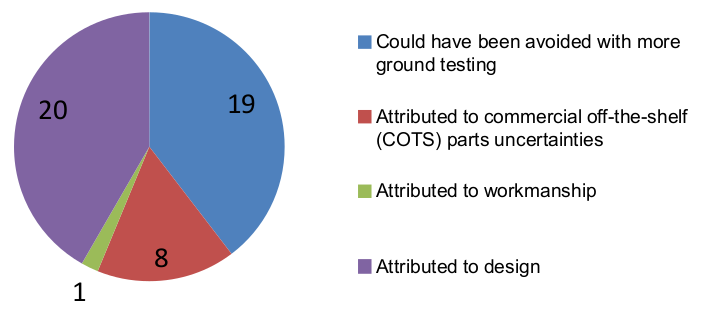
\includegraphics[height=4.5cm]{figure/cause_of_failure.png}
      \caption{故障原因に関するインタビュー結果\cite{Venturini2017}}
      \label{fig:cause of failure}
\end{figure}

%ここへのつながり
また,大学衛星が商用利用や革新的なミッションに
挑戦するためには,超小型衛星のメリットである
コストの低さを十分に確保しながら,
ほどよい信頼性を実現することが,重要であると考えられている\cite{SHIRASAKA2011}.\\
故障に設計や製造の不良が含まれていることを考えると,
超小型衛星の「ほどよい信頼性」の評価を行うためには,
従来用いられてきた
各コンポーネントごとの信頼度の組み合わせでは不十分である.
そこで,設計・製造・運用における
信頼度を加味した評価手法が提案されている\cite{SHIRASAKA2011}.
式(\ref{eq:Reliability})が示すように,この評価手法では
製造時の信頼性も重要な要素であると捉えられている.

\begin{equation}
   R_{sat} = R_{des} \times R_{fab} \times R_{comp} \times R_{op} \label{eq:Reliability}
\end{equation}
\begin{table}[H]
   \centering
      \begin{tabular}{cl} 
        $R_{sat}$ & 衛星の真の信頼度\\
        $R_{des}$ & 設計における信頼度\\
        $R_{fab}$ & 製造における信頼度\\
        $R_{comp}$ & 衛星の信頼度(従来の信頼度)\\
        $R_{op}$ & 運用における信頼度
      \end{tabular}
\end{table}

%もうちょいちゃんと考える
\subsection{地上試験における問題}
以上で示したように,不具合の多くが設計,製造などに起因している
という問題がある.
一方で,これは超小型衛星開発のみに限られたことではなく,
中・大型衛星においても大きな問題となっている.
軌道上故障データを分析した結果\cite{SAITO2011}(Figure \ref{fig:error tyoe})
によると,軌道上で
偶発的に発生した故障はわずか11%であり,それ以外は設計,製造などの開発
活動に起因するものであることがわかっている.\\
また,軌道上で発生した不具合が地上試験で
発現しなかった,または発見できなかった原因が以下の
Figure \ref{fig:error cause}のように知られている.
試験設備の不足によるものや,故障発見までの
時間が長く試験で発見することが現実的で無いものに関しては,
コストとリソースの面から試験による対策では限界がある.
一方で,試験モードの不備や,発現していたのにもかかわらず
発見できなかった不具合に関しては
試験に対する習熟度が不足していること,
不具合・リスクの分析が不十分であることが推測される\cite{SAITO2011}.

\begin{figure}[H]
   \centering
      \begin{tabular}{c}
         \begin{minipage}{0.50\hsize}
         \centering
         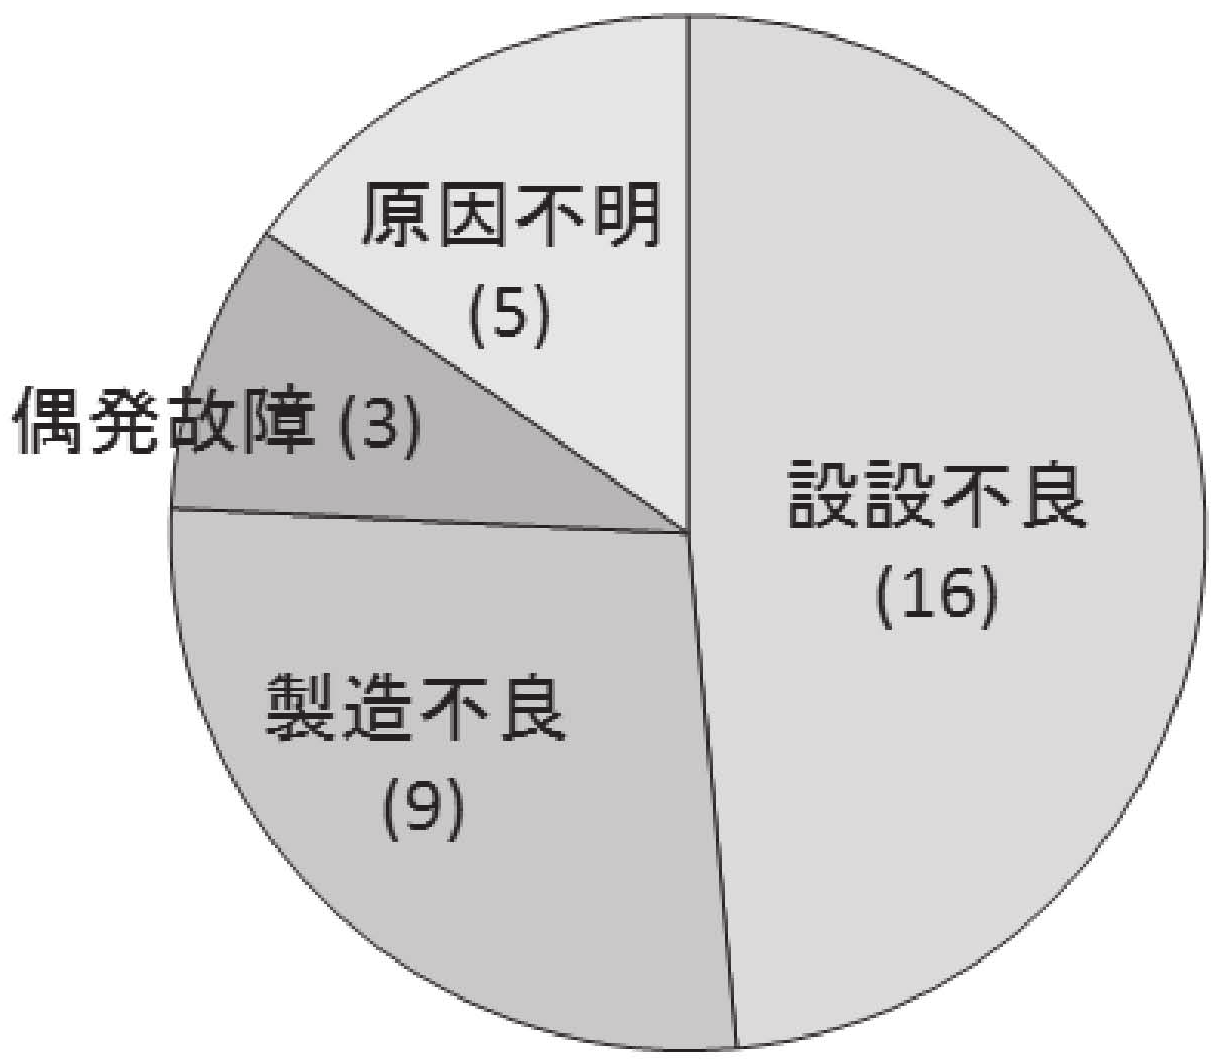
\includegraphics[width=5.5cm]{figure/on_orbit_error_tyoe.png}
            \caption{軌道上故障の原因類型の分布\cite{SAITO2011}}
            \label{fig:error tyoe}
         \end{minipage}
         \begin{minipage}{0.50\hsize}
         \centering
         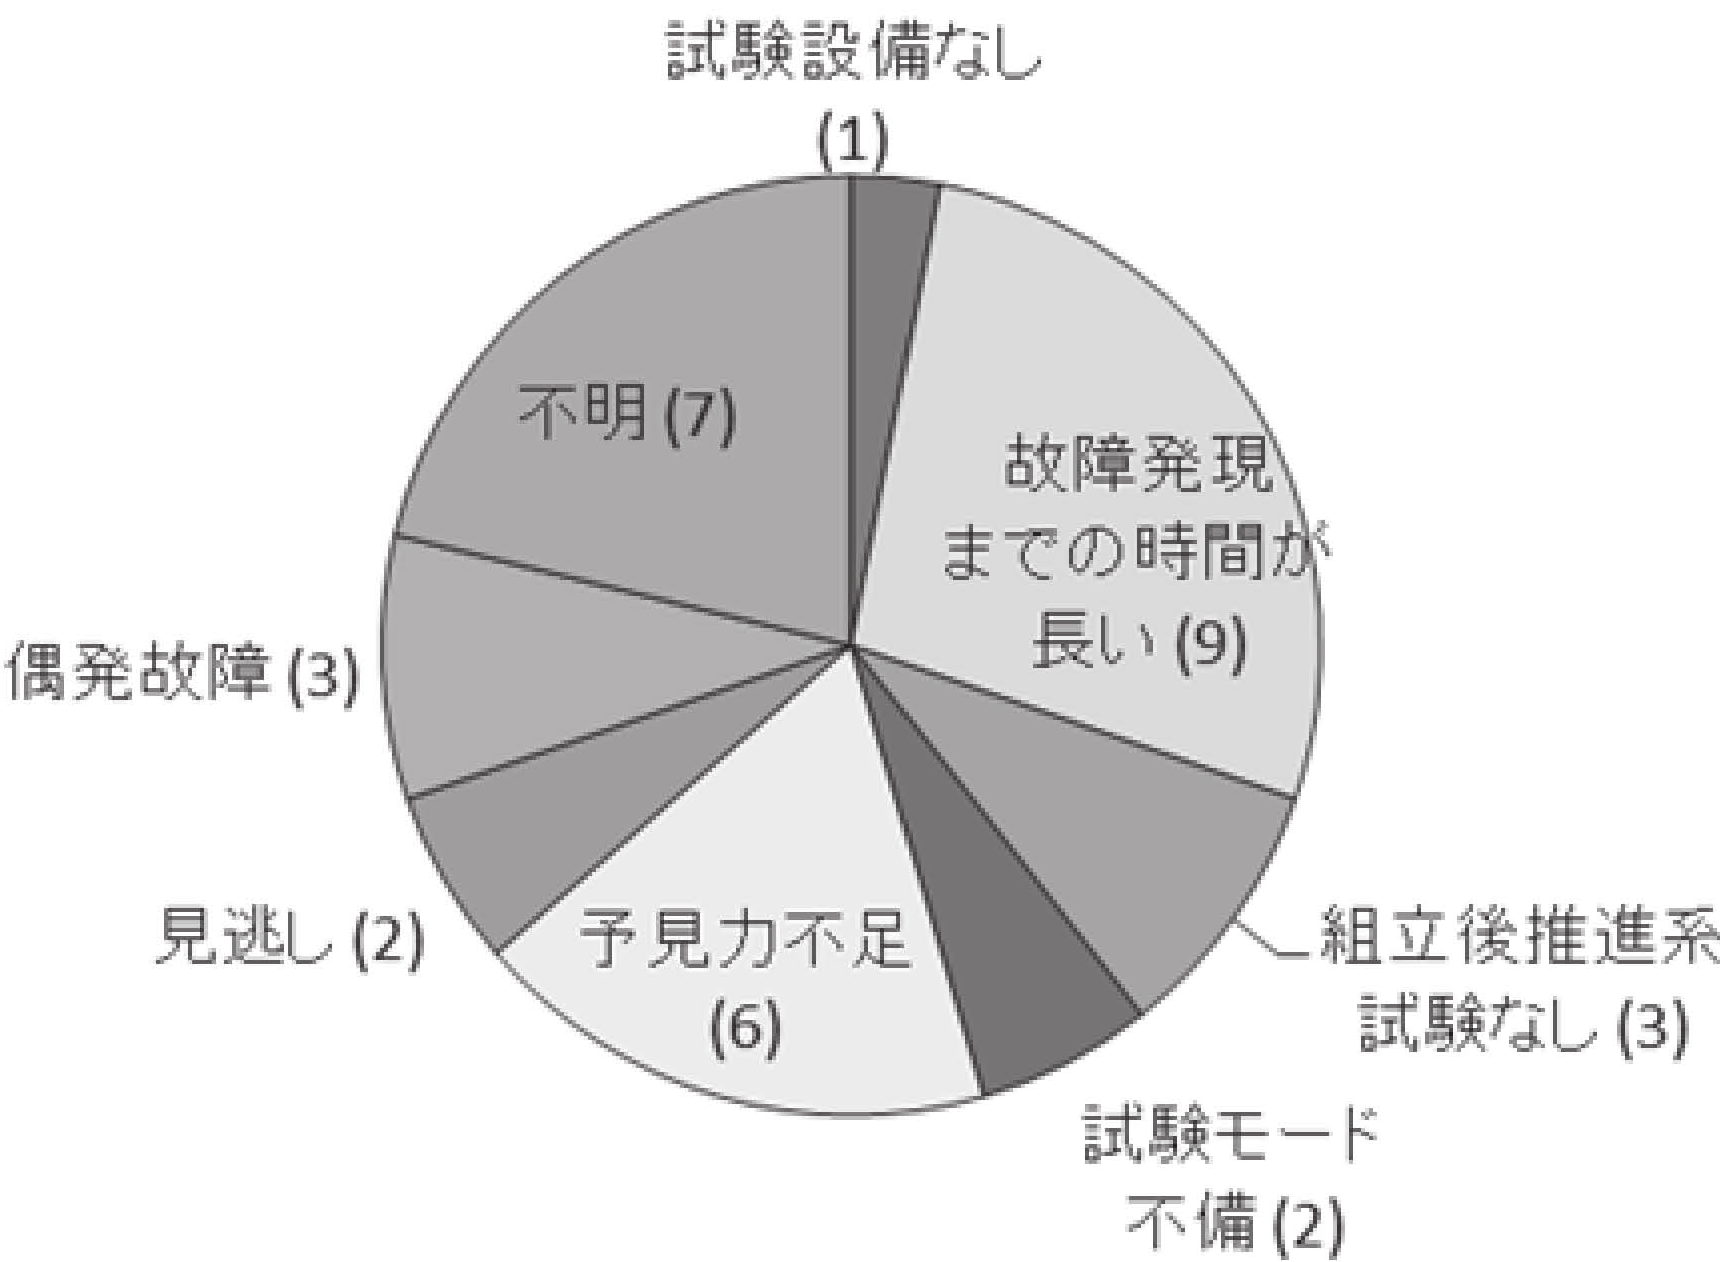
\includegraphics[height=5.5cm]{figure/not_found_error_seeds.png}
            \caption{軌道上故障の要因を地上で発見できなかった原因類型の分布\cite{SAITO2011}}
            \label{fig:error cause}
         \end{minipage}
      \end{tabular}  
\end{figure}


%ここを不具合分析の難しさに変える.
%なぜこの研究室で不具合の分析が十分に行えていなかったのかをFTA使って分析したものをベースに考えよう.
%ここの流れを見直す.根拠資料
\subsection{不具合分析の難しさ}
以上のように,衛星の不具合及びリスク分析を,
地上試験で十分に
行うことができていないという現状がある.\\
以下に人による不具合原因分析の大まかな流れを示す.
\begin{enumerate}
   \item 不具合が起きた際の衛星の状態を保存する. %これ試験の話と軌道上での話が混じってる
   \item テレメトリから考えられる故障原因の候補を洗い出す.
   \item それらの故障の中でテレメトリから分かる情報を元に候補を棄却していく.
   \item 更に切り分けが必要な場合はコマンドを送って,それに影響を受けるテレメトリによって判断する.
   \item 判断できない場合は,コンポーネントを取り出し直接確認を行う.
\end{enumerate}
分析が不十分になっている原因の一つとして,2の故障原因の候補
の洗い出しを網羅的に行うことの難しさがある.
組み上げ状態の衛星から得られる情報はテレメトリのみである.
この際,衛星の内部状態を理解し,テレメトリから現在の衛星の状態
を想像することができなければ,十分に不具合の原因の候補を考えることはできない.
本研究室の過去プロジェクト(PRISM)を対象にした研究では,
事前に想定していた故障モードの粒度は,
%ここの記述も微妙なので変更する
山口ら\cite{Yamaguchi2014}がモデルを用いて洗い出したものと比較して,
不十分であるという結果も出ている.
このように,人による故障モードの洗い出しは思いつきによるものなので,
考えが及んでいないことが多い.\\
また,分析が不十分になっている原因の一つとして,
3,4の故障原因の切り分け作業の難しさもある.
超小型衛星は内部状態が複雑に絡み合っており,一つの不具合に対して
非常に多くの故障候補が洗い出されることが想像できる.
そのため,多くの故障候補の中から切り分けを行い,最終的な故障を
特定するという作業は多くの知識と労力を必要とする作業である.
%この時,未熟な運用者が原因特定のために誤ったコマンドを送信してしまうと,
%衛星が死ぬ可能性も考えられる.このため,不具合分析を行う際には
%そのコマンドが”安全”なのかという点が非常に重要となる.


\section{本研究での目的}
以上を踏まえると,
不具合発生時に故障候補を洗い出し,その切り分けを行って
原因を特定していく過程に,高い知識と経験が必要になっている
ことが,
衛星の不具合やリスクの分析が不十分に
なっている原因の一つであると言える.

% 提案手法へのつながりが見えにくいため,違う記法の方がいいかもしれない.
そこで本研究では,経験が浅く,衛星に関する知識の乏しいエンジニアであっても
不具合分析を実施できるような不具合分析支援の手法を提案する.
この手法は下記の3つの要素で構成されている.
\begin{itemize}
   \item 衛星内部のサブシステムや要素間の信号・電気・物理的相互作用のモデル化
   \item コマンド及びテレメトリによって情報が流れる経路のモデル化
   \item 不具合原因の特定を行うために必要なコマンド及びテレメトリ
   の探索 %ここの言い回し
\end{itemize}
   
まずは,簡易的な衛星のモデルに対してテストケースを考え,
手法の有効性を検証し,有効であることが十分に示すことができれば,
本研究室における衛星開発で部分的に実践し有効性を
検証することを考えている.\\

\section{先行研究調査}
モデルを元に不具合診断を行うシステムの研究は古くから行われており,\cite{}
正常時のコンポーネント間のつながりモデルに基づく不具合分析
手法としてGDEが一般的である.
推論時に扱うことのできる

以下に比較結果を示す.
\begin{table}[H]
   \centering
   \caption{不具合分析手法の比較}
      \begin{tabular}{cccccc} \hline
         手法&網羅範囲&故障仮説生成&仮説検証支援&モデル化コスト%これは微妙かもしれない
         \\
         GDE\cite{}&\\
         GDE+\cite{Struss1989}&\\
         \cite{Yamaguchi2014}&\\
         \cite{Kitamura1999}&\\
         本手法&&&\\
      \end{tabular}
\end{table}

詳細なモデルを用いて,不具合原因である機器の故障の原因などを探索可能にしたものなど
あるが,網羅的な故障仮説の洗い出しを行うことがメインであり,
実際の検証段階を組み込んだものは少ない.


故障診断の全ての過程を対象の制約モデルを用いて行うことは,
対象とするモデルの粒度に非常に高い忠実度が求められるため,複雑に物理現象が絡み合う
衛星では難しい.
むしろ,人間を対話的にサポートすることによってシステムに求められるモデル化のコスト
を下げつつ,不具合分析(故障診断)の過程を体系化し,経験の少ないエンジニアの支援が
できると考えられる.


本手法では,衛星へのアクションとしてコマンドを用いながら,故障仮説の洗い出しと
検証を同時に行うことによって,用意すべきモデルに求められる粒度のレベルを下げている.
%こんな感じかな....

自分の手法の新規性を示す.

%以下で何を書くかをまとめる
%まずは手法の説明
%コマンドを評価するための指標に関して
%探索のアルゴリズムの具体的説明
%実装結果.モデルの説明も必要になる(できればわかりやすい形で示したい)
%探索結果に関する考察
%




\section{現在の状況}
以下では,現在検討しているモデル化の手法に関して
述べたあと,ケーススタディを用いて
本手法による具体的な不具合分析の流れを説明する.

\subsection{提案手法}
以下のFigure \ref{fig:fault_diagnosis}に提案手法の不具合分析を行うフローを示す.
図中において本研究の対象は,黄色に示しているところであり,
不具合発生時のコマンド送信情報とテレメトリ情報
が与えられてから,それらが通る経路の探索を行い,その経路内に
存在する故障箇所を検証するために必要な確認事項の洗い出しを行うことである.

%図は修正する
%どこからどこの間がおかしいということを示すことができる.具体的に何がおかしいのかはまた別の話
\begin{figure}[H]
   \centering
      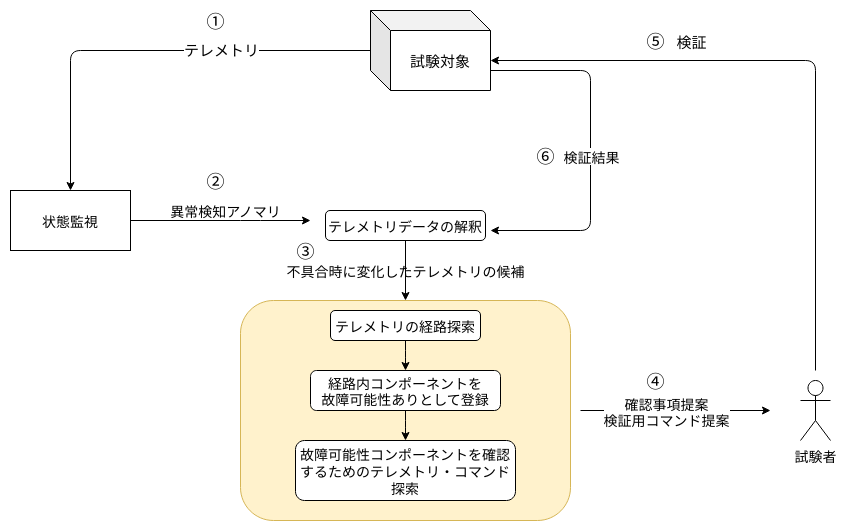
\includegraphics[height=8.0cm]{figure/fault_diagnosis_flow.png}
      \caption{不具合分析の流れ}
      \label{fig:fault_diagnosis}
\end{figure}

本手法の不具合分析の流れは以下である.
\renewcommand{\labelenumi}{\roman{enumi}}
\begin{enumerate}
   \item 不具合検知のきっかけとなったテレメトリの候補を与える.
%   どこが異常値なのかを認識させる. 
   %不具合を起こしたトリガーが何なのかは分からないが,コマンドによってもたらされたかの区別だけ必要?
   \item そのテレメトリに影響を与えるコマンドを送信してから,
   地上局がテレメトリを受信するまでの一連の経路を取得する.
   \item 得られた経路内にあるコンポーネント,配線などを故障候補として登録する.
   %その経路に対してコマンドパスとして入力があれば,入力の元となっているコンポーネントも故障候補に追加する.
   \item 他のテレメトリを確認することによって,棄却できる故障候補を棄却する.
   \item コマンドを送って得られるテレメトリ情報によって,
   故障候補の検証ができるコマンドの探索を行う.
   \item 以上で得られたコマンドを,人が安全性などを考慮した上で実行し故障候補の切り分けを行う.\\
\end{enumerate}



また,上記のアルゴリズムによって切り分けを行うためのコマンドを評価する指標として以下のもの
を考えた.
%指標に関する説明
%運用時における話をしていないのにいきなり出てくるとおかしいような気がする.
地上試験と運用時の両方で使い分けることのできるフレームワークであることを示す.
地上試験時は,不具合の切り分けを十分に行いたいので,確実な箇所から切り分けを行うこと
を考える.確実に切り分けを行っていくためには,コマンドによって変化する状態量
が少ないことが望ましい.

制約の違い
電力を考慮するのか,など

可視時間が限られていて,そのパス中に不具合原因を究明しなければいけないような時間制約
がある場合がある.その際には,効率的に切り分けが行えるコマンドである必要がある.
その指標として,コマンドの能力を情報量の定義から考えた.

\begin{eqnarray}
   P_i = \frac{Command number which can verify port i}{All command number}\\
   I_j = -\sum_{i_j} \log{P_{i_j}}      
\end{eqnarray}

このようなアルゴリズムで不具合分析を行うためには,
以下のようなモデルが必要となることがわかった.
\begin{itemize}
   \item 各コンポーネント間の接続関係
   \item コマンド・テレメトリがコンポーネント間を伝わる経路
   \item コマンドに影響を受けるテレメトリの関係
\end{itemize}

\subsection{モデル化手法}
以上で述べた,不具合分析に必要になるモデルの構築方法に関して
具体的なテストケースを用いて現在の検討状況を述べる.
\subsubsection{対象とするテストケース}
今回,以下のFigure \ref{fig:simple_sat}の
ような簡易衛星モデルを考え,モデル化の手法について
述べる.\\
また,矢印の色が情報の方向性を表しており
赤がコマンドによる情報の伝達過程,
青がテレメトリによる情報の伝達過程である.
また,矢印の種類が情報として伝わる物
を表しており,それぞれ以下のようになっている.
\begin{itemize}
   \item Signal:電気信号
   \item Radio wave:電波
   \item Power:電源
   \item Heat:熱
\end{itemize}
\begin{figure}[H]
   \centering
      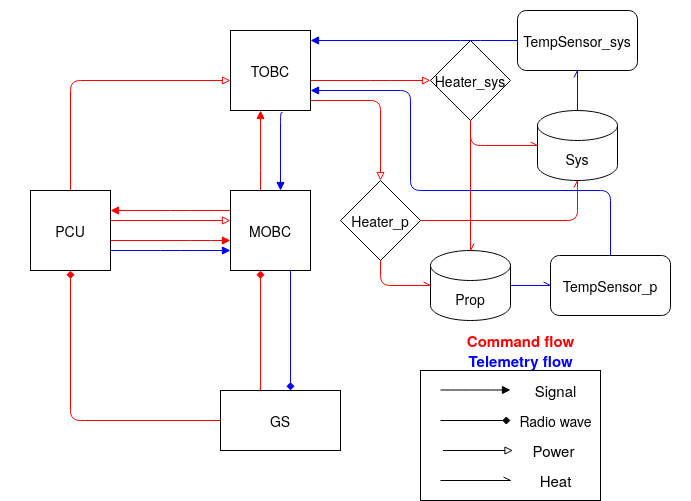
\includegraphics[height=9.0cm]{figure/simple_sat.png}
      \caption{簡易衛星モデル}
      \label{fig:simple_sat}
\end{figure}

\subsubsection{各コンポーネント間の接続関係の構築方法}
山口ら\cite{Yamaguchi2014}は人工衛星デバイスオントロジーとして,
衛星内部でのコンポーネント間のつながりを表現するために「ポート」
という概念を定義している.この手法を参考にし,以下のTable \ref{tab:port_definition}
ポートの定義を行い,Table \ref{tab:compo_port}のように各コンポーネント
の属性としてポートを定義した.\\
ポートが持つ情報としては,ポート名,接続コンポーネント,ID,伝達物
となっており,IDが各ポート固有の識別子としてポートを参照する際に
使用される.接続コンポーネントが同一の場合でも,Table \ref{tab:port_definition}
のID:4.1,4.2のように伝達物が異なるものは別ポートとして定義し,IDによって区別
を行う.

\newpage
%キャプションとくっついているか確認
\begin{table}[H]
   \centering
   \caption{ポート定義} 
   \label{tab:port_definition}
\end{table} 
\vspace{-2zh}
\begin{figure}[H]
   \centering
      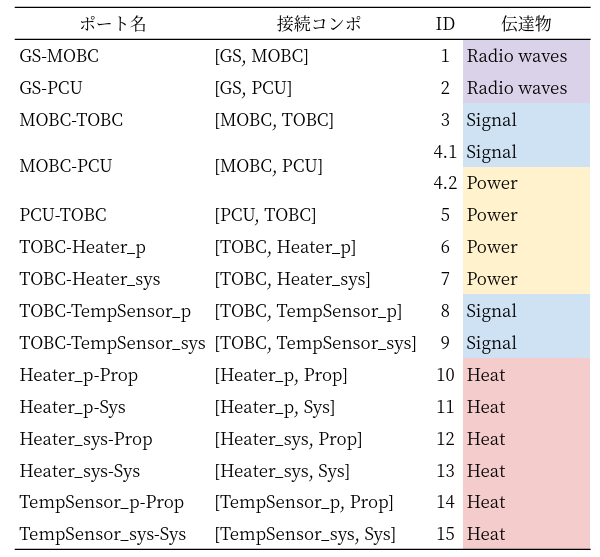
\includegraphics[height=10cm]{figure/port_definition.png}
\end{figure}
次に,コンポーネントの定義を行う.以下のTable \ref{tab:compo_port}では,
衛星システム全体として使用されている
コンポーネントのリストを作成し,各コンポーネントの属性として
コマンドポートとテレメトリポートを,上で定義したポートのID
を用いて定義している.
ここで,コマンドポートというのはコマンドの経路で使用されるポートであり,
テレメトリポートというのはテレメトリの伝達で使用されるポートである.
この時,属性として持つポートはそのコンポーネントが出力元となる場合としている.

%キャプションとくっついているか確認
%\newpage
\begin{table}[H]
   \centering
   \caption{コンポーネント定義} 
   \label{tab:compo_port}
\end{table}
\vspace{-2zh}
\begin{figure}[H]
   \centering
      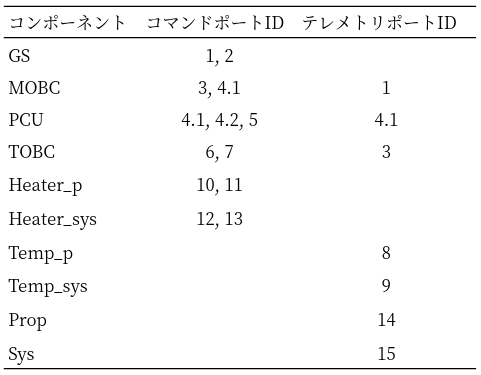
\includegraphics[height=7cm]{figure/compo_port.png}
\end{figure}

以上の情報によって,衛星内部でコンポーネント全体がどのように接続しているか
を定義することが可能になる.
また,コマンド及びテレメトリが伝達していく
経路のモデルは,以上の情報からコンポーネントとポートを順に
辿っていくことによって構築することが可能であると考えている.

\subsubsection{コマンド・テレメトリがコンポーネント間を伝わる経路の構築方法}
次に,コマンド及びテレメトリがコンポーネント間を伝わる経路を探索するために
必要なコマンド及びテレメトリの定義に関して述べる.
まず,今回の衛星モデルにおいて使用できるテレメトリ及びコマンド
を以下のTable \ref{tab:telemetry},\ref{tab:command}に示す.

\begin{table}[H]
   \centering
   \caption{使用テレメトリ}
   \label{tab:telemetry}
      \begin{tabular}{cllcccc} \hline
         ID&テレメトリ&経路\\ \hline
         1&MOBCカウンター&MOBC$\rightarrow$GS\\
         2&MOBC電流値&PCU$\rightarrow$MOBC$\rightarrow$GS\\
         3&TOBCカウンター&TOBC$\rightarrow$MOBC$\rightarrow$GS\\
         4&TOBC電流値&PCU$\rightarrow$MOBC$\rightarrow$GS\\
         5&推進系温度&Prop$\rightarrow$TempSensor\_p$\rightarrow$TOBC$\rightarrow$MOBC$\rightarrow$GS\\
         6&システム温度&Sys$\rightarrow$TempSensor\_sys$\rightarrow$TOBC$\rightarrow$MOBC$\rightarrow$GS\\
         7&推進系ヒータ電流値&TOBC$\rightarrow$MOBC$\rightarrow$GS\\
         8&システムヒータ電流値&TOBC$\rightarrow$MOBC$\rightarrow$GS\\
         9&MOBCコマンドカウンター&MOBC$\rightarrow$GS\\
         10&TOBCコマンドカウンター&TOBC$\rightarrow$MOBC$\rightarrow$GS\\ \hline
      \end{tabular}
\end{table}

%ここも修正
\begin{table}[H]
   \centering
   \caption{使用コマンド}
   \label{tab:command}
      \begin{tabular}{clllccc} \hline
         ID&コマンド&経路&影響テレメトリID\\ \hline
         1&MOBC電源ON&GS$\rightarrow$PCU$\rightarrow$MOBC&1,2,9\\
         2&MOBCコマンドカウンターアップ&GS$\rightarrow$MOBC&9\\
         3&TOBCコマンドカウンターアップ&GS$\rightarrow$MOBC$\rightarrow$TOBC&10\\
         %3&MOBCテレメトリダウンリンク&GS$\rightarrow$MOBC&1,2,3,4\\
         %4&TOBCテレメトリダウンリンク&GS$\rightarrow$MOBC$\rightarrow$TOBC&5,6,7,8\\
         %3&TOBCの温度計データダウンリンク&GS$\rightarrow$MOBC$\rightarrow$TOBC&5,6\\
         \multirow{2}{*}{4}&\multirow{2}{*}{推進系ヒータON}&GS$\rightarrow$MOBC$\rightarrow$PCU$\rightarrow$TOBC&\multirow{2}{*}{5,6,7}\\
         &&$\rightarrow$Heater\_p$\rightarrow$(Prop,Sys)&\\
         \multirow{2}{*}{5}&\multirow{2}{*}{システムヒータON}&GS$\rightarrow$MOBC$\rightarrow$PCU$\rightarrow$TOBC&\multirow{2}{*}{5,6,8}\\
         &&$\rightarrow$Heater\_sys$\rightarrow$(Prop,Sys)&\\
         6&TOBC電源ON&GS$\rightarrow$PCU$\rightarrow$TOBC&3,4,10\\ \hline
      \end{tabular}
\end{table}

Table \ref{tab:telemetry}に示すテレメトリの経路及び,Table \ref{tab:command}
に示す経路と影響テレメトリIDを上で定義したコンポーネントの接続関係のモデル
から探索したい.
各コマンドとテレメトリの定義情報として,情報伝達の始点と終点を定義しておき,
端点から接続関係モデルを用いて探索すること
で経路を構築できないか検討している.%これ以上は時間次第,練習して行けそうなら入れる.
%一方で,上位層ではいくつかのパターンが存在する.これを上手く認識させる方法がないか模索中.
\begin{comment}
   カテゴリーという概念を用いることで,経路を構築するために
必要な情報の粒度を単純化できると考えている.
カテゴリーはコマンドやテレメトリの経路の中でGSから最も遠くにあるOBCによって定義する.
これによって,多くのコマンド及びテレメトリが共通して通るGS−各OBC間の経路
を,事前に定義したものから接続することが可能になる.
例を挙げると,コマンドID:4 推進系ヒータONコマンドは「TOBCカテゴリー」,
テレメトリID:2 MOBC電流値は「PCUカテゴリー」となる.\\
カテゴリーは衛星を構成するOBCの種類だけ存在し,
今回のモデルであれば以下のOBCカテゴリーが存在する.
\begin{itemize}
   \item MOBC
   \item PCU
   \item TOBC
\end{itemize}

\end{comment}

%ここはほんまは受信機があるやんけ,この概念意味なさそう・・
%今回の問題設定では意味ある..改善事項ということで発表すればええ
%ココらへん簡単にまとめる.検討段階ということでええ
%コマンドの種類によって最上位OBCという概念を導入する.
%\begin{itemize}
%   \item 信号系コマンド:MOBC
%   \item 電源系コマンド:PCU
%\end{itemize}


%懸念事項をここに書いておく

%一つのコマンド及びテレメトリの定義時に必要となる情報を以下に例を用いて示す.
%ここにコマンドとテレメトリの定義情報を載せる.

\subsubsection{コマンドに影響を受けるテレメトリの関係}
Table \ref{tab:command}に各コマンドが影響を与えるテレメトリの
IDを定義しており,この関係によってコマンドを打った際に得られる
情報を類推することが可能になる.\\
この関係を,コンポーネント間の接続関係モデルと
コマンド・テレメトリの経路情報などから生成できると考えている.
%どうする?
例えば,
コマンドの終点とテレメトリの始点が一致しているものがこの関係性にある
ことが多くある.
%こういうコメントなくす
しかし,一意的にこの方法で定義することは難しく,
コマンド経路の途中にあるコンポーネントから波及して
影響を受けるテレメトリも存在するため,さらなる検討が必要である.

%コマンドの種類によっては送信しアクションを起こさないもの

\subsection{各故障を切り分けていくための確認事項の探索}
次に,故障候補の中から切り分けを行っていくためのアルゴリズムに関して
検討状況を述べる.
不具合が発生している状態で予期せぬ二次故障を起こさないために,
探索順序としては,
衛星の状態を変えずに確認できるものを優先的に探索
することが望ましい.\\
%ここ表現がわかりにくい
そこで,不具合発生時に取得しているテレメトリデータの中から
故障原因特定に役に立つテレメトリ情報が存在するなら,
そのテレメトリを確認事項として提案する.

また,衛星の状態変化を行わずに
故障原因特定のために得られる情報がなくなれば,
次ステップとしてコマンドを打って得られる
情報から切り分けを行っていくことになる.このとき,
対象となるコマンドが通る経路の中で,地上局(Ground Station,GS)の近く
の経路から順に,検証を行うためのコマンドの探索を行う.

\subsection{問題設定}
最後に,不具合分析の具体的な流れをみるために,以下のような故障を考え,
不具合分析を行っていく.\\
まず,MOBCとTOBCからテレメトリは全て降ろされているものと仮定する.
また,故障は「推進系ヒータの接着不良」であるとする.
その時,テレメトリを通して確認できるのは
\begin{itemize}
   \item 「推進系ヒータON」コマンドを送ったのに,「推進系温度」テレメトリが変化しない.
\end{itemize}
という事象である.
よって不具合検知は,この事象によって行われる.

\subsubsection{不具合分析の例}
この不具合において,「推進系ヒータON」コマンドを送信して推進系ヒータに熱が伝わるまでの経路
と,推進系温度計が温度を読み取り「推進系温度」テレメトリとして地上局に伝わるまでの
経路の中に故障箇所があると考えることができる.
この経路を以下のFigure \ref{fig:simple_sat_fault}に太矢印で示している.
%これにポートID入れたら見やすいかも
\begin{figure}[H]
   \centering
      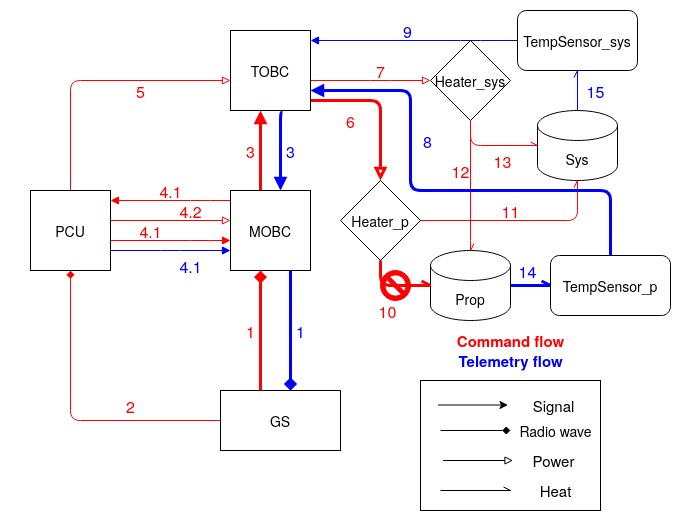
\includegraphics[height=9.0cm]{figure/simple_sat_fault.png}
      \caption{故障箇所と不具合検知に関連するコマンドとテレメトリの経路}
      \label{fig:simple_sat_fault}
\end{figure}
また,この経路内にあるコンポーネントに電源が入っているかどうかを確認するためには,
そのコンポーネントに電源を供給するための経路が正常に作動しているかどうかを確認する
必要がある.そこで
\begin{itemize}
   \item PCU$\rightarrow$MOBC(ポートID:4.2),PCU$\rightarrow$TOBC(ポートID:5)
\end{itemize}
も検証を行う対象として考える.
以上より,検証すべき経路は下記のようになる.
\begin{itemize}
   \item コンポーネント:GS,MOBC,TOBC,Heater\_p,Prop,TempSensor\_p
   \item コマンドポート:GS-MOBC(1),MOBC-TOBC(3),MOBC-PCU(4.2),
   PCU-TOBC(5),\\TOBC-Heater\_p(6),Heater\_p-Prop(10)
   \item テレメトリポート:GS-MOBC(1),MOBC-TOBC(3),TOBC-TempSensor\_p(8),
   TempSensor\_p-Prop(14)
\end{itemize}
以下,提案手法によるアルゴリズムによって不具合分析を行っていく.\\
%この章長くて読みにくい
まず,問題設定よりMOBC及びTOBCのテレメトリは全てダウンリンクされている状態に
あるので,
\begin{itemize}
   \item テレメトリポート:TOBC$\rightarrow$MOBC(3),MOBC$\rightarrow$GS(1)
   \item コマンドポート:PCU$\rightarrow$MOBC(4.2),PCU$\rightarrow$TOBC(5)
\end{itemize}
は問題ないことが確認できるため,故障可能性はなくなる.
問題設定ではあるが,実際に「MOBC及びTOBCのテレメトリが全てダウンリンクされている」
ことを確認するためには,「MOBCカウンター」
「TOBCカウンター」を確認することが必要である.\\
また不具合発生時,推進系ヒータが正常に作動しており,
システム温度計からテレメトリを下ろす経路に問題がなければ,
「システム温度」が上昇しているはずである.
よって,テレメトリの確認によって検証できる経路として,
コマンドポート「TOBC-Heater\_p(6)」がある.
以上より,不具合発生時から状態変化させずに確認すべき事項として以下
が挙げられる.

\begin{table}[H]
   \centering
   \caption{コマンドなしでの確認事項} 
   \label{tab:check_list1}
\end{table}
\vspace{-2zh}
\begin{figure}[H]
   \centering
      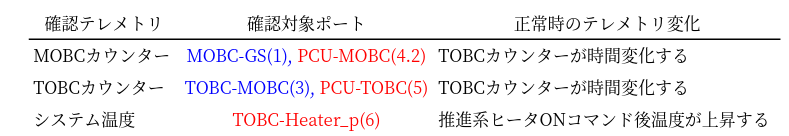
\includegraphics[height=2.5cm]{figure/check_list_tel.png}
\end{figure}
衛星の状態を変化させること無く,テレメトリを確認するだけで
検証できる箇所はこれ以上存在しないので,次にコマンドによる検証を行う.

まず,コマンドパスとしてGSに近い箇所から順に確認を行う必要がある.
MOBCへのコマンドが通っているかを確認するためには,「MOBCコマンドカウンターアップ」
コマンドを送って,「MOBCコマンドカウンター」が変化していることを確認できれば良い.
同様に考えると,以下の様に確認事項を洗い出すことができる.
\begin{table}[H]
   \centering
   \caption{コマンド送信による確認事項} 
   \label{tab:check_list2}
\end{table}
\vspace{-2zh}
\begin{figure}[H]
   \centering
      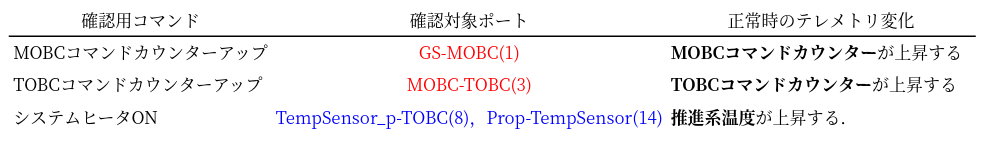
\includegraphics[height=2.6cm]{figure/check_list.png}
\end{figure}
以上の項目を確認した際,今回想定した故障モード(推進系ヒータの接着不良)
では期待されるテレメトリデータの変化が起こるので,
Table \ref{tab:check_list2}の確認対象パスの中にある故障可能性箇所は
棄却され,
故障可能性ポートとして残るのは
\begin{itemize}
   \item コマンドポート:Heater\_p-Prop(10)
\end{itemize}
となる.

%上のコマンドを送っても大丈夫なのかという議論はどうするのか?もしシステム温度が高いのに,その方法でたしかめてもいいものなのか?

この経路上で考えうる故障モードと照らし合わせると,
この切り分けによって残る故障モードは
\begin{itemize}
   \item 推進系ヒータの故障
   \item 推進系ヒータの接着不良
\end{itemize}
となる.
この時,
「システム温度」の上昇によって「推進系ヒータの故障」の可能性は
棄却できるため,最終的に「推進系ヒータの接着不良」
が残り,
実際の故障を棄却すること無く,絞り込みができていると言える.\\
%以上の不具合分析の流れを参考にし,探索のアルゴリズムを考えたい.
\section{今後の方針}
今後は,上のような不具合分析の流れをモデルを元に行うことができるように,
簡易的なものを作成し,検証していく.

また,生成された確認事項を実行するに当たって,衛星の状況によっては
コマンドを打つことで衛星が危険に晒されることも考えられる.
最終的には,コマンドが安全であるかどうかという判断基準も試験を行う人に
対して明示できると良いと考えている.\\
また,熱や運動のような支配方程式が微分方程式で定義されており,
単純なつながりだけでは表現できないような現象に関しては,
この手法では簡易的に表現することしかできていない.
そのため,この手法を物理現象が複雑に絡んだ不具合分析に適用することは難しい.
将来的には,これらの支配方程式を解く
シミュレータを組み込むことによって複雑な物理現象も扱えるように
手法の改良が必要である.

\bibliographystyle{junsrt} %何がええかは考える plain, acm, alpha とか
\bibliography{Ref} 
\end{document}